\documentclass[a4paper,12pt,notitlepage,spanish,final]{report} % Imprime por un solo lado de la hoja
%\documentclass[letterpaper,12pt,notitlepage,spanish,final,twoside]{report} % Imprime por los dos lados de la hoja
\usepackage{algorithm}
\usepackage[noend]{algorithmic}
\usepackage{amsfonts}
\usepackage[centertags]{amsmath}
\usepackage{amssymb}
\usepackage{amsthm}
\usepackage[spanish]{babel}
\usepackage[margin=12pt,font=small,labelfont=bf,labelsep=endash,skip=10pt]{caption}
\usepackage{dsfont}
\usepackage[dvips]{epsfig}
\usepackage[mathcal]{euscript}
\usepackage{float}
\usepackage{slashbox}
%\usepackage{graphics}
%\usepackage{graphicx}
\usepackage{hyperref}
\usepackage[latin1]{inputenc}	% ISO-8859-1 codificaci�n en espa�ol (incluye acentos)
%\usepackage[utf8]{inputenc}	% Codificaci�n est�ndar en ingl�s
\usepackage{newlfont}
% Para incluir el Glosario. Notar que se debe compilar usando: "makeindex tesis.nlo -s nomencl.ist -o tesis.nls" (orden: pdflatex, makeindex y pdflatex)
\usepackage[intoc, refpage]{nomencl}	
\usepackage{subfig}
\usepackage{sty/utfsm_tesis}
\usepackage{upgreek}
\usepackage{url}
\usepackage[table]{xcolor}
\usepackage{xtocinc}		% Include Table of Contents as the first entry in TOC
\usepackage{listings}
\lstset{ %
  language=Java
  }
% ---------------------------------------------------------------------------------------------------------------
% Fuzz
\hfuzz 2pt
\hoffset -1.0in		% Seteo a 0 el margen izquierdo
%\oddsidemargin 4cm		% Margen izquierdo (pag. impar)
\oddsidemargin 3cm	% Ancho Legal 21,59cm
\evensidemargin 0.5cm	% Alto Legal 35,56cm
\textwidth 15.5cm
\topmargin -1.5cm
%\voffset 2cm 		% Margen superior
\textheight 22cm
%\parindent 0em
%\parskip 2ex
\newlength{\defbaselineskip}
\setlength{\defbaselineskip}{\baselineskip}
\newcommand{\setlinespacing}[1]
           {\setlength{\baselineskip}{#1 \defbaselineskip}}
\newcommand{\doublespacing}{\setlength{\baselineskip}
                           {1.3 \defbaselineskip}}
\newcommand{\singlespacing}{\setlength{\baselineskip}{\defbaselineskip}}
% ---------------------------------------------------------------------------------------------------------------
% F�rmulas matem�ticas utilizadas
\newcommand{\bbbr}{\mathbb R}
\hyphenation{de-no-mi-na-das} \hyphenation{co-rres-pon-den}
\hyphenation{ha-bi-tual-men-te} \hyphenation{ins-tan-cias}
\hyphenation{con-glo-me-ra-do} \hyphenation{an-te-rior-men-te}
\hyphenation{co-rres-pon-dien-te} \hyphenation{ins-truc-cio-nes}
\hyphenation{am-bien-tes}  \hyphenation{re-pre-sen-ta-cion}
\hyphenation{pre-sen-cia}
% Teoremas
\theoremstyle{plain}
\newtheorem{hipot}{Hip�tesis}[chapter]
\newtheorem{thm}{Teorema}[section]
\newtheorem{cor}[thm]{Corolario}
\newtheorem{lem}[thm]{Lema}
\newtheorem{prop}[thm]{Proposici�n}
\newtheorem{defn}{Definici�n}[section]
\theoremstyle{remark}
\newtheorem{rem}{Observaci�n}[section]
\numberwithin{equation}{section}
\renewcommand{\theequation}{\thesection.\arabic{equation}}
\floatname{algorithm}{Algoritmo}
% ---------------------------------------------------------------------------------------------------------------
\setlength{\tclineskip}{1.05\baselineskip}
% ---------------------------------------------------------------------------------------------------------------
\newcommand{\anc}{5.1cm}
\newcommand{\alt}{5.1cm}
\newcommand{\M}{{\mathcal M}}
\newcommand{\ra}{\rightarrow}
\newcommand{\converge}[2]{\underset{#1 \ra #2}{\ra}}
\newcommand{\limite}[2]{\underset{#1 \ra #2}{\lim}}
\newcommand{\deriv}[2]{\frac{\partial{#1}}{\partial{#2}} }
\newcommand{\ve}{\varepsilon}
\newcommand{\V}{{\mathcal V}}
\newcommand{\E}{{\cal E}}
\newcommand{\norm}[1]{\left\Vert#1\right\Vert}
\newcommand{\abs}[1]{\left\vert#1\right\vert}
\newcommand{\eps}{\varepsilon}
\newcommand{\s}[1]{{\mathbf #1}}
\newcommand{\ol}{\overline}
\newcommand{\Real}{{\mathbb R}}
\newcommand{\C}{{\mathcal C}}
\newcommand{\W}{{\mathcal W}}
\newcommand{\D}{{\mathcal D}}
\newcommand{\minimo}[1]{\underset{#1}{\min}}
\newcommand{\thetaM}{\hat{\s{\theta}}_n^M}
\newcommand{\I}{\mathcal{I}}
\newcommand{\N}{\mathcal{N}}
\newcommand{\Hip}{\mathcal{H}}
\newcommand{\ms}[1]{\mathbf{#1}}
% ---------------------------------------------------------------------------------------------------------------
%Redefinici�n de comandos del paquete "algorithmic"
\renewcommand{\algorithmicwhile}{\textbf{Mientras}}
\renewcommand{\algorithmicfor}{\textbf{Para}}
\renewcommand{\algorithmicdo}{\textbf{hacer}}
\renewcommand{\algorithmicend}{\textbf{fin}}
% ---------------------------------------------------------------------------------------------------------------
% Redefinici�n de comandos del paquete "nomencl".
\renewcommand{\nomname}{Glosario}
\renewcommand{\pagedeclaration}[1]{. Ver p�gina~\hyperpage{#1}.} % Usar este comando en conjunto con el paquete "hyperref"
\makeatletter % necesario para que reconozca a '@' como car�cter normal 
\renewcommand{\paragraph}{\@startsection{paragraph}{4}{\z@}{-3.25ex \@plus 
-1ex \@minus -.2ex}{1.5ex \@plus .2ex}{\normalfont\normalsize\bfseries}} 
\makeatother % necesario para que restablezca '@' como car�cter especial
\makenomenclature %Genera el Glosario
% ---------------------------------------------------------------------------------------------------------------
\DeclareGraphicsExtensions{.pdf,.png,.jpg}
\graphicspath{{./img/}}

% ---------------------------------------------------------------------------------------------------------------
\begin{document}
% Opciones del Documento.
%\draft %Notar que la numeraci�n cambia, dejando los n�meros de p�gina en la parte superior (a no ser que sea comienzo de cap�tulo).
%\nobib
%\nofront
%\nolistoftables \nolistoffigures
% ---------------------------------------------------------------------------------------------------------------
%\magister
\begin{center}
\ingciv
\copyrightyear{2014}
\submitdate{\today}
\convocation{Julio}{2014}
% ---------------------------------------------------------------------------------------------------------------
\title{An�lisis de herramientas para mejorar la calidad de aplicaciones para Android}
\author{Cristopher Nicol�s Oyarz�n Altamirano}
\end{center}

%\twosupervisors
\profguia{Cecilia Reyes}
\profcorr{Chihau Chau}
%\profext{por definir} %Solo Magister
\ack{tex/00.0-agradecimientos} % Incluir Agradecimientos
\dedicate{``Dedicado a mis padres, Guillermo y Alicia, que se han sacrificado por darme el mejor de los regalos, la educaci�n"}	
\resumenesp{tex/00.1-resumen}			% Incluir Resumen (Espa�ol)
\resumening{tex/00.2-abstract}			% Incluir Abstract (Ingl�s)
\abreviaciones{tex/00.3-glosario}		% Incluir Glosario

%\WinEdt{?0000} % Don't bother with over/under-full boxes
% ---------------------------------------------------------------------------------------------------------------
\setcounter{tocdepth}{3}
\beforepreface
%\WinEdt{?1111} % Process all errors from here on
\afterpreface
% ---------------------------------------------------------------------------------------------------------------
% Introducci�n de la Tesis
% ---------------------------------------------------------------------------------------------------------------
\chapter{Introducci�n}
\label{cha:intro}

\section{Definici�n del problema}
\label{sec:problematica}

\section{Objetivos}
\label{sec:objetivos}
\subsection{Objetivo principal}

\subsection{Objetivos espec�ficos}
\begin{itemize}
\item item
\end{itemize}

\section{Estructura del documento}
\label{sec:estructura}

%Introducci�n			\ref{ch:intro} 
%Estado del Arte		\ref{ch:eda} 
%Herramientas Actuales	\ref{ch:herram}
%Analisis comparativo	\ref{ch:analis}
%implementaciones		\ref{ch:implem}
%Conclusiones			\ref{ch:conc}
%Ap�ndice A				\ref{ch:apeA}
%Ap�ndice B				\ref{ch:xxxx}
% ---------------------------------------------------------------------------------------------------------------
% Estado del Arte
% ---------------------------------------------------------------------------------------------------------------
\definecolor{dkgreen}{rgb}{0,0.6,0}
\definecolor{gray}{rgb}{0.5,0.5,0.5}
\definecolor{mauve}{rgb}{0.58,0,0.82}

\lstset{frame=tb,
  language=Java,
  aboveskip=3mm,
  belowskip=3mm,
  showstringspaces=false,
  columns=flexible,
  basicstyle={\small\ttfamily},
  numbers=none,
  numberstyle=\tiny\color{gray},
  keywordstyle=\color{blue},
  commentstyle=\color{dkgreen},
  stringstyle=\color{mauve},
  breaklines=true,
  breakatwhitespace=true
  tabsize=3
}

\chapter{Estado del Arte}
\label{ch:eda}

En este cap�tulo se dar� a conocer el estado actual de la cartera energ�tica de Chile, en la cual se encuentra trabajando el gobierno de Chile en conjunto con distintas agencias gubernamentales y no-gubernamentales, espec�ficamente en el �rea de la Eficiencia Energ�tica. En conjunto con esto, se dar� a conocer las distintas metodolog�as de los procesos de toma de decisiones multicriterio que se utilizan en la actualidad.

\section{Referencia del Sector Energ�a}
El sector de energ�a es estrat�gico y fundamental para el funcionamiento de nuestra sociedad y la vida de las personas. La energ�a es una fuente necesaria para el uso de artefactos el�ctricos, de calefacci�n y cocina, as� como tambi�n para el transporte y el funcionamiento del sector productivo.


El contexto mundial y nacional de las tres �ltimas d�cadas es radicalmente distinto del
escenario que se proyecta para los pr�ximos treinta a�os. Los hidrocarburos (carb�n, petr�leo y gas) se presentaban hasta hace unos a�os como una fuente de energ�a abundante, barata y respuesta preferente a los desaf�os que el desarrollo econ�mico mundial requer�a. Sin embargo, la creciente urbanizaci�n mundial y la irrupci�n de nuevos pa�ses como grandes consumidores de energ�a, probablemente implicar� un panorama m�s complejo de escasez y alta competencia por el uso de algunos combustibles, mayor volatilidad y altos precios de la energ�a. Las emisiones de contaminantes locales y globales de los hidrocarburos son una raz�n adicional para disminuir la dependencia de los combustibles f�siles y buscar nuevas fuentes energ�ticas propias, m�s limpias y a precios accesibles

\subsection{Energ�a en Chile}
Chile importa el 60\% de su energ�a primaria (Balance Nacional de Energ�a BNE 2012), por lo que somos un pa�s subordinado a la inestabilidad y volatilidad de los precios en los mercados internacionales y las restricciones de abastecimiento que se produzcan por fen�menos pol�ticos, clim�ticos o de mercado.\\

Los �ltimos diez a�os en Chile han estado marcados por el corte de gas natural desde Argentina, severos y largos per�odos de sequ�a, dificultades en el otorgamiento de permisos ambientales, insuficiente entrada de proyectos y de nuevas empresas en el �rea de generaci�n y escasa inversi�n en infraestructura en ese mismo segmento y tambi�n en transmisi�n el�ctrica. Todo ello ha contribuido a sostener a lo largo de la �ltima d�cada condiciones de estrechez de oferta de suministro el�ctrico, con altos costos marginales y precios a cliente final que reflejan un desarrollo ineficiente del sistema, lo que se ha agravado en los �ltimos a�os.\\

En efecto, los precios de la energ�a el�ctrica han aumentado considerablemente en la �ltima d�cada. En 2006, el suministro el�ctrico para el pueblo chileno, comercios y peque�as empresas (clientes regulados) fue adjudicado a valores promedio de US\$ 65 por MWh; en cambio, la �ltima licitaci�n, realizada en diciembre de 2013 para estos mismos clientes, fue adjudicada al doble del 2006 (valor promedio de US\$ 128 por MWh). Esto ha significado que la cuenta el�ctrica que pagan hoy las familias chilenas es un 20\% superior respecto al a�o 2010. De mantenerse el escenario de precios adjudicados en 2013, el costo de la electricidad podr�a subir otro 34\% durante la pr�xima d�cada.\\

Asimismo, en los �ltimos diez a�os, las industrias (clientes libres) han visto duplicados los precios por sus consumos el�ctricos, lo que resta competitividad a nuestra econom�a e impacta directamente en el crecimiento del PIB. En el a�o 2013, los precios medios de mercado rondaron en el Sistema Interconectado Central (SIC) los US\$ 112 por MWh y en el Sistema Interconectado del Norte Grande (SING) los US\$ 108 por MWh. La industria chilena est� enfrentando uno de los precios m�s altos de la energ�a el�ctrica en Am�rica Latina. En el caso de la miner�a, el sector enfrenta el segundo precio m�s alto con respecto a los pa�ses mineros a nivel mundial, y el doble con respecto a competidores directos, como Per�.

\subsection{La Eficiencia Energ�tica (EE) en Chile}

\subsection{Ministerio de Energ�a}

\subsection{Innovaci�n y Desarrollo Tecnol�gico en EE en Chile}

\subsubsection{Fundaci�n Chile}

\subsubsection{Superintentencia de Electricidad y Combustibles (SEC)}


\section{Toma de decisiones Multicriterio y Metodolog�a}

\subsection{Conceptos}

\subsection{Metodolog�a AHP}

\subsection{Metodolog�a ANP}
%!TEX root = ../tesis.tex
% Cap?ulo 3: Herramientas Actuales
% ---------------------------------------------------------------------------------------------------------------
\chapter{Marco Metodol?ico}
\label{ch:herram}

\section{Metodolog? para el modelamiento e implementaci? de las soluciones}

\section{Herramientas de Modelamiento}
\subsection{Herramientas de Proceso Anal?ico Jer?quico (AHP)}
\subsection{Herramientas de Proceso Anal?ico en Red (ANP)}
% Cap�tulo 4: An�lisis Comparativo
% ---------------------------------------------------------------------------------------------------------------
\chapter{An�lisis Comparativo}
\label{ch:analis}

% Cap�tulo 5: Implementaci�n
% ---------------------------------------------------------------------------------------------------------------
\chapter{Implementaci�n}
\label{ch:implem}

En este cap�tulo se realizar� la implementaci�n de las herramientas m�s destacadas en base a los an�lisis previos. La integraci�n de estas herramientas se llevar�n a cabo en un entorno real de desarrollo, espec�ficamente en la aplicaci�n \textbf{Seahorse} \cite{55}. Esta aplicaci�n est� enfocada en la creaci�n colaborativa y privada de albumes de fotos y v�deos. En la figura \ref{fig:Fig20} es posible ver algunas de las pantallas de esta aplicaci�n.
\begin{figure}[h!]
\centering
      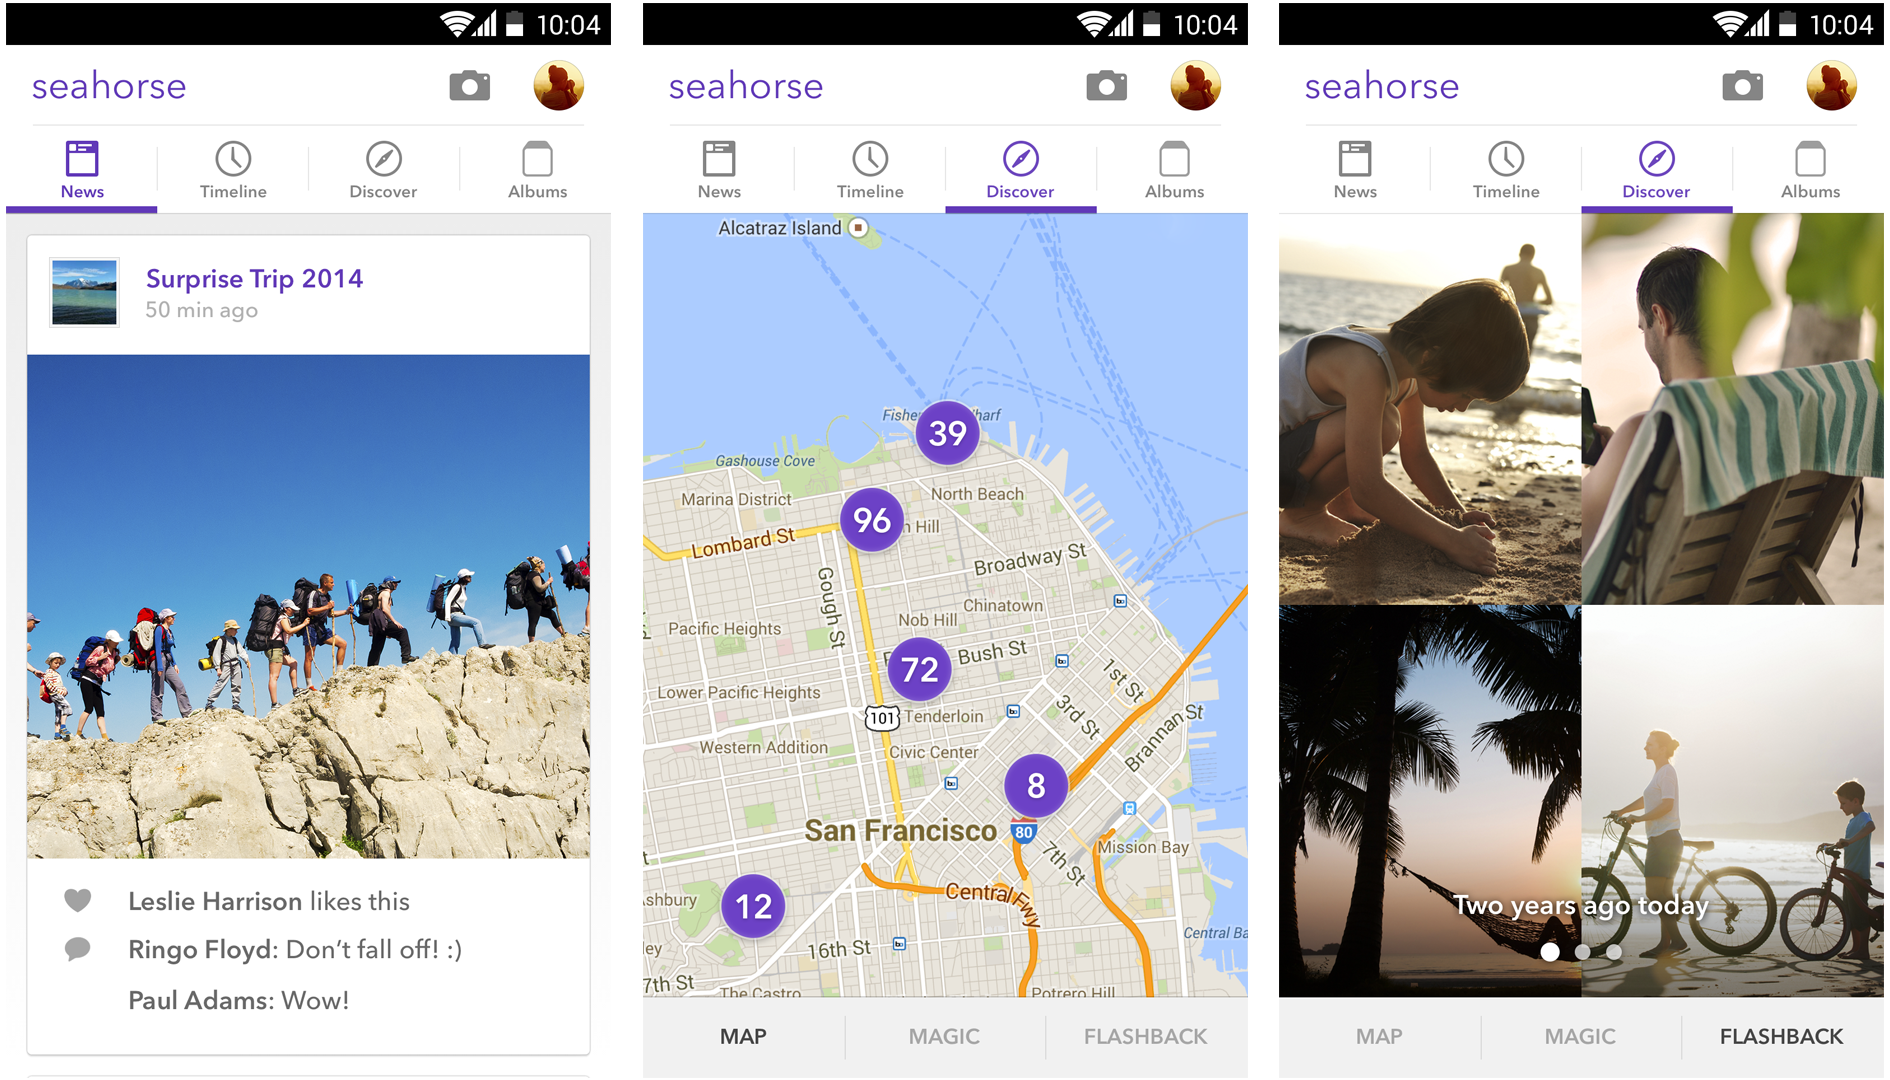
\includegraphics[width=15cm]{Imagenes/seahorse_screenshots}
\caption{Vistas de la aplicaci�n Seahorse. Fuente: Elaboraci�n Propia}
\label{fig:Fig20}
\end{figure}

Las herramientas implementadas son las que m�s se ajustaban a las necesidades y a los recursos con los que cuenta Seahorse, por lo que f�cilmente este conjunto de herramientas puede diferir en relaci�n a las implementaciones que otros desarrolladores har�an en sus aplicaciones.

\section{Implementaci�n de Herramientas de Testing}
\subsection{Robolectric}
Para la implementaci�n de Robolectric es necesario seguir los pasos de instalaci�n que se detallan en su sitio oficial \cite{56}. En Seahorse se usa Gradle \cite{61} para automatizar la construcci�n y compilaci�n el proyecto, aunque tambi�n es posible usar Ant \cite{62} o Maven \cite{63}. Para agregar Robolectric a un proyecto configurado con Gradle es necesario agregar esta l�nea al archivo \textit{build.gradle} del proyecto:
\begin{lstlisting}
dependencies {
  ...
  androidTestCompile 'org.robolectric:robolectric:2.3' 
}
\end{lstlisting}
Para m�s detalles sobre c�mo realizar la instalaci�n con Android Studio, se puede seguir el tutorial que presenta en su blog \cite{57} uno de los desarrolladores de Google.

El test que se llev� a cabo consiste en verificar que el flujo inicial de la aplicaci�n se realice de forma correcta. B�sicamente se testea que el usuario pueda acceder sin problemas a las pantallas de login y de registro. En la figura \ref{fig:Fig21} se muestra el flujo que se someter� a prueba, el cual consta de 3 tareas b�sicas:
\begin{itemize}
\item Abrir Seahorse.

\item Presionar el bot�n que dice \textit{Log In} y mostrar un men� con opciones.

\item Presionar el bot�n que dice \textit{Sign in with email} y llevar al usuario a la vista de Login.
\end{itemize}

\begin{figure}[h!]
\centering
      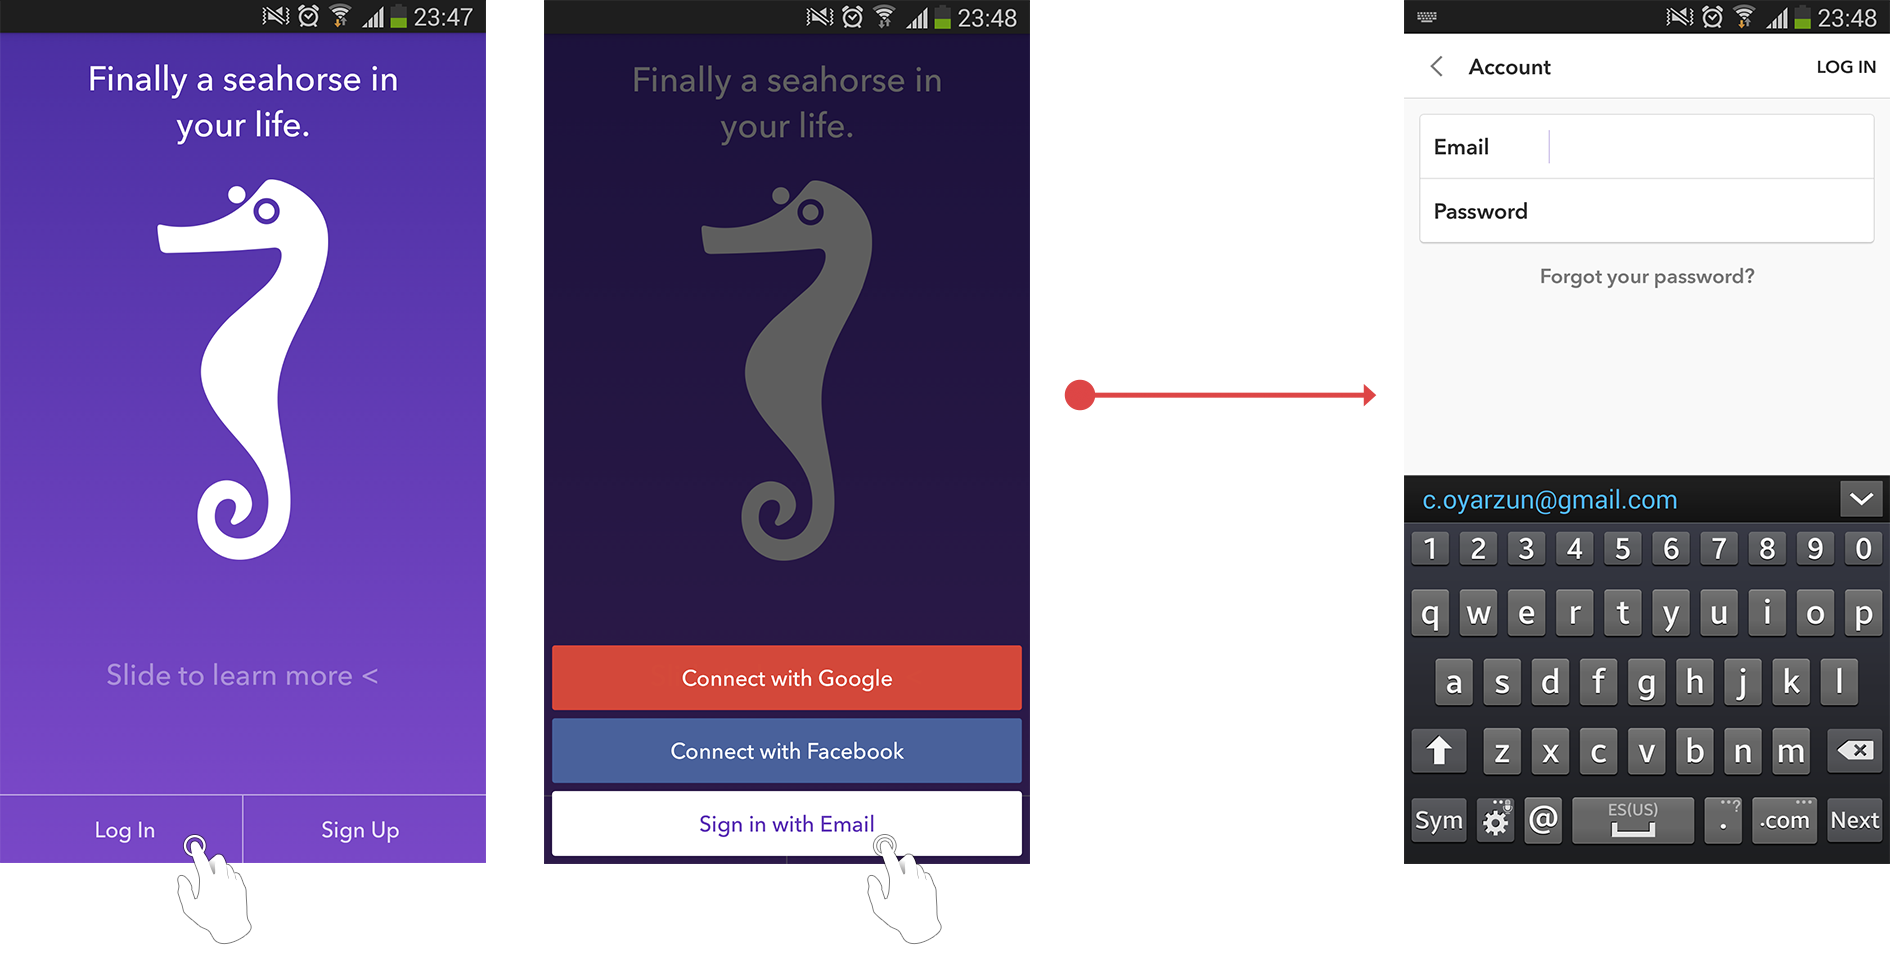
\includegraphics[width=15cm]{Imagenes/seahorse_testing_flujo_login}
\caption{Flujo para acceder a la pantalla de Login en la aplicaci�n Seahorse. En la primera imagen se presiona el bot�n \textit{Log In}, lo cual abre el menu de la segunda imagen, y se presiona el bot�n \textit{Sign in with email}, lo que abre la vista de Login de la �ltima imagen. Fuente: Elaboraci�n Propia}
\label{fig:Fig21}
\end{figure}

Dentro del proyecto de Seahorse, se cre� una clase en el paquete \textit{co.seahorse.android.test}. En este caso la \textit{Activity} testeada es SeahorseStartActivity y el nombre de la clase que se encarga de realizar el test es SeahorseStartActivityTest. 
\begin{lstlisting}
@RunWith(RobolectricGradleTestRunner.class)
public class SeahorseStartActivityTest {
    private SeahorseStartActivity activity;
    private Button buttonLogin;
    private Button buttonRegister;
    private Button buttonSign;
    @Before
    public void setup() throws Exception {
        activity = Robolectric.buildActivity(SeahorseStartActivity.class).create().
            start().get();
        buttonLogin = (Button) activity.findViewById(R.id.buttonLogInAccount);
        buttonRegister = (Button) activity.findViewById(R.id.buttonRegisterAccount);
        buttonSign = (Button) activity.findViewById(R.id.buttonSignIn);
    }
\end{lstlisting}
El m�todo \textit{setup()} se encarga de crear la referencia a la \textit{Activity} que se desea testear y obtener los botones que tambi�n ser�n testeados.

Es una buena pr�ctica verificar que ninguno de los elementos obtenidos en el m�todo anterior est�n vac�os, por lo que el primer test se encargar� de eso:
\begin{lstlisting}
    @Test
    public void shouldNotBeNull() {
        assertNotNull(activity);
        assertNotNull(buttonLogin);
        assertNotNull(buttonRegister);
        assertNotNull(buttonSign);
    }
\end{lstlisting}

Por �ltimo se realiza el test del flujo que lleva a la pantalla de Login:
\begin{lstlisting}
    @Test
    public void buttonClickShouldStarLoginActivity() throws Exception {
        buttonLogin.performClick();
        buttonSign.performClick();
        Intent intent = Robolectric.shadowOf(activity).peekNextStartedActivity();
        assertEquals(LoginActivity.class.getCanonicalName(), intent.getComponent().getClassName());
    }
    \end{lstlisting}
A trav�s del m�todo \textit{performClick()} es posible simular la l�gica del bot�n, tal como si un usuario real lo hubiese presionado. Esto se realiza dos veces, ya que se tienen que simular dos clicks a dos botones distintos. El �ltimo de los click es el que se encarga de abrir la pantalla de Login, por lo que se obtiene el Intent creado por este click a trav�s del m�todo \textit{peekNextStartedActivity()}, para luego verifica a trav�s del m�todo \textit{assertEquals} que la \textit{Activity} que se inici� corresponda a \textit{LoginActivity}.

Al ejecutar los tests, se genera un reporte en HTML, que se ubica en la ra�z del proyecto, en \textit{./build/test-report/index.html}. En este reporte se detalla la cantidad total de test ejecutados y el tiempo que se demoraron, como tambi�n los test que fallaron y la raz�n.

\subsection{Robotium}
Se implement� Robotium, en vez de Espresso, principalmente porque existe mayor documentaci�n y porque cuenta con soporte para gradle de forma oficial, por lo que la integraci�n con Android Studio es menos compleja. Adem�s lleva m�s tiempo de desarrollo y es una herramienta bastante madura.

Para agregar Robotium a un proyecto configurado con Gradle es necesario agregar esta l�nea al archivo \textit{build.gradle} del proyecto:
\begin{lstlisting}
dependencies {
  androidTestCompile 'com.jayway.android.robotium:robotium-solo:4.3'
}
\end{lstlisting}
El test que se realiz� es similar al realizado a trav�s de Robolectric, aunque ahora de forma instrumental, es decir ejecut�ndolo directamente en el dispositivo. Para ello se ha creado la clase RobotiumTest, la cual consiste en lo siguiente:
\begin{lstlisting}
public class RobotiumTest extends ActivityInstrumentationTestCase2 {
    private Solo solo;
    public RobotiumTest() {
        super(SeahorseStartActivity.class);
    }

    public void setUp() throws Exception {
        super.setUp();
        solo = new Solo(getInstrumentation(), getActivity());
    }

    public void testRobotium()  throws Exception {

        solo.assertCurrentActivity("SeahorseStartActivity Never Loaded", SeahorseStartActivity.class);
        solo.clickOnText(getActivity().getString(R.string.LOGIN));
        solo.waitForText(getActivity().getString(R.string.SIGN_IN_WITH_EMAIL));
        solo.clickOnText(getActivity().getString(R.string.SIGN_IN_WITH_EMAIL));
        solo.assertCurrentActivity("LoginActivity Never Loaded", LoginActivity.class);
        solo.takeScreenshot();
    }
\end{lstlisting}
La clase \textit{Solo} es la principal para desarrollar tests con Robotium. En el m�todo \textit{setup()} se crea una referencia de \textit{Solo} a partir de la \textit{Activity} actual.

En el m�todo \textit{testRobotium()} es donde se lleva a cabo el test. Como se puede ver, todo se realiza a trav�s de la clase \textit{Solo}. Con ella se corrobora en un principio si la \textit{Activity} actual corresponde a \textit{SeahorseStartActivity}, luego se hace un click en el texto que dice ``Log In''. Debido a que existe una animaci�n para mostrar el men�, se recurre al m�todo \textit{waitForText} para esperar que la animaci�n termine y luego presionar este bot�n. Finalmente se presiona el texto ``Sign in with email'' y se comprueba que la nueva \textit{Activity} corresponda a \textit{LoginActivity}. Todo este proceso, al ser ejecutado en un dispositivo real, demora 5.69 segundos, lo cual no es mucho, pero si se toma en cuenta que dentro de un proyecto se puede tener una gran cantidad de tests, entonces s� puede decirse que es un tiempo considerable. Debido a esto, es importante decidir de forma sabia, qu� cosas son realmente necesarias testear de manera instrumental.

%\subsection{Espresso} 
%Para la implementaci�n de Espresso, uno de los mayores problemas es que no cuenta oficialmente con soporte para gradle, por lo que se utiliz� la biblioteca Double Espresso \cite{58}, que no cambia en nada el c�digo original y simplemente le agrega este soporte. Las dependencias agregadas a gradle son:
%\begin{lstlisting}
%dependencies {
%  ...
%  androidTestCompile 'com.jakewharton.espresso:espresso:1.1-r3'
%  androidTestCompile 'com.jakewharton.espresso:espresso-support-v4:1.1-r3'
%}
%\end{lstlisting}
%A diferencia de Robolectric, Espresso se especializa en los test relacionados con la interfaz de la aplicaci�n. 
\subsection{Spoon}
Spoon es una herramienta que intenta simplificar la tarea de realizar tests de forma distribuida. Es posible ejecutar los mismos tests escritos con Robotium en m�ltiples dispositivos simult�neamente. Una vez que todos los tests se han completado, un resumen es presentado con informaci�n detalla sobre cada dispositivo y cada test en un archivo HTML.

Es necesario agregar dos archivos al proyecto, uno es \textit{spoon-runner} que permite la ejecuci�n simult�nea, y el otro es \textit{spoon-client} que se encarga de obtener screenshots de cada uno de los dispositivos, para luego presentarlos en el resumen general.

Para realizar el testing de forma distribuida fue usado un dispositivo Samsung Galaxy S4 y dos emuladores. Debido a que los emuladores provistos por Android son demasiados lentos se usaron los de Genymotion \cite{64}. Ellos ofrecen cerca de 20 emuladores con las simulaciones de distintos dispositivos de forma gratuita. En este caso se usaron los emuladores de un Nexus 4 con Android 4.2.2 y un HTC One con 4.2.2.

El test que se realiz� consist�a en corroborar que en la pantalla de registro, al completar los datos y dejar uno en blanco, si se presiona el bot�n ``SIGN UP'', debe aparecer un �cono en el campo vac�o, indicando que se necesita completar toda la informaci�n. Para ello se utiliz� Robotium junto con Spoon, el primero para poder interactuar con la UI, mientras que Spoon se utiliz� para obtener los screenshots de los tres dispositivos durante todo el proceso. El c�digo a continuaci�n muestra el uso de Spoon, a trav�s del m�todo \textit{Spoon.screenshot}:
\begin{lstlisting}
    Spoon.screenshot(getActivity(), "RegisterActivity");
    solo.assertCurrentActivity("SeahorseStartActivity Never Loaded", RegisterActivity.class);
    solo.enterText((EditText) solo.getView(R.id.editLastNameRegister), "Oyarzun");
    solo.enterText((EditText) solo.getView(R.id.editEmailRegister), "c.oyarzun@gmail.com");
    solo.enterText((EditText) solo.getView(R.id.editPasswordRegister), "123456");
    Spoon.screenshot(getActivity(), "RegisterActivityWithInfo");
    solo.clickOnText(getActivity().getString(R.string.SIGN_UP).toUpperCase());
    Spoon.screenshot(getActivity(), "ShowMissingField");
\end{lstlisting}
Una vez que el test ya est� listo, es necesario ejecutar por l�nea de comandos lo siguiente:
\begin{lstlisting}
   cristopher$ java -jar spoon-runner-1.1.1-jar-with-dependencies.jar --apk ../PhotoApp/build/outputs/apk/PhotoApp-debug.apk --test-apk ../PhotoApp/build/outputs/apk/PhotoApp-debug-test-unaligned.apk --sdk ../../../Downloads/adt-bundle-mac-x86_64/sdk/
\end{lstlisting}
Los par�metros que se agregan son: el APK, el APK del test y la ruta del SDK. Despu�s de unos segundos se genera una carpeta con el nombre \textit{spoon-out} que contiene los resultados de los tests en cada uno de los dispositivos. 

En la figura \ref{fig:Fig24} se pueden ver los resultados obtenidos en el emulador de Genymotion Nexus 4, en el dispositivo Samsung S4 y en el emulador Genymotion HTC One. Todos los test funcionaron de forma correcta, aunque en la �ltima pantalla, si bien se muestra el �cono indicando que el campo est� vac�o, �ste deber�a estar acompa�ado de un di�logo con un texto con el mensaje ``This field is required'', por lo que se puede ver que Spoon no es capaz de capturar los di�logos que se muestran sobre la \textit{Activity} testeada.

\begin{figure}
\centering
      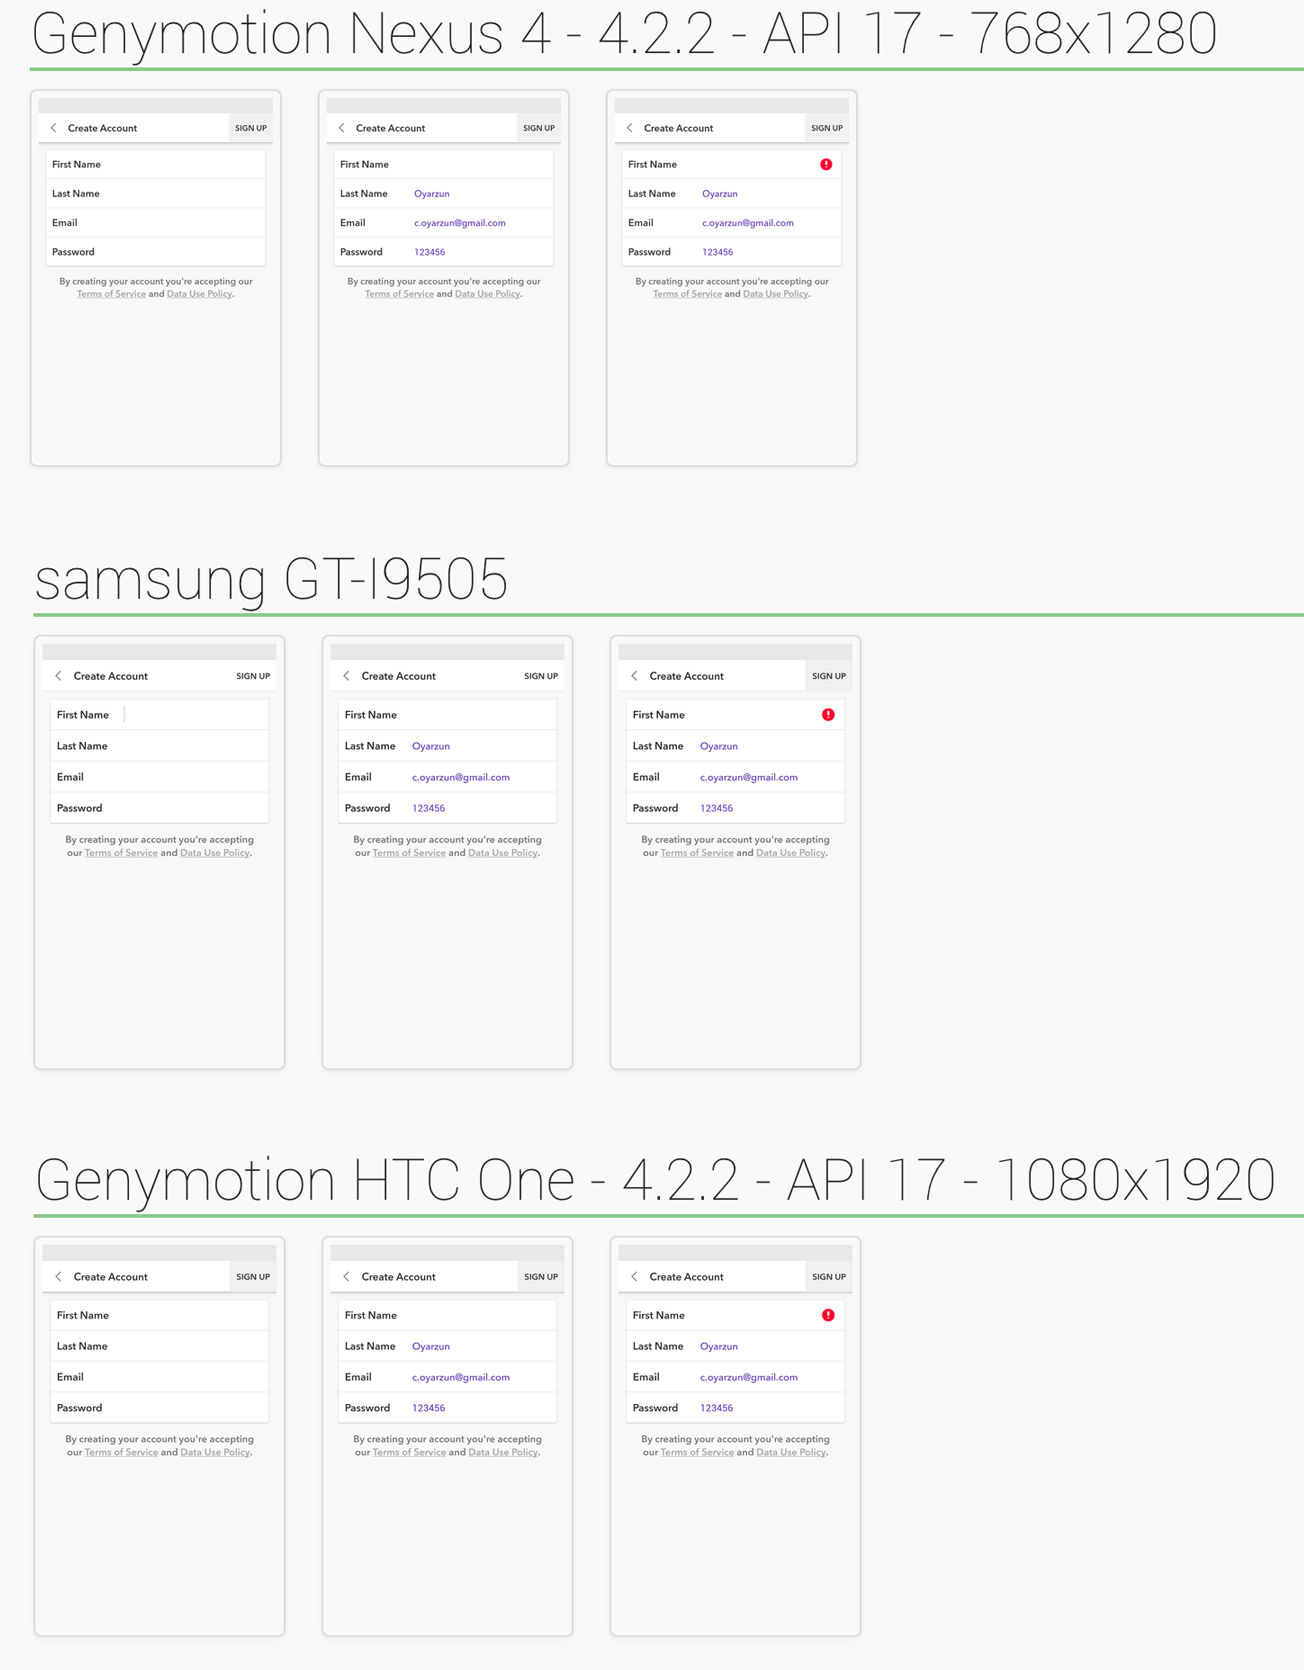
\includegraphics[width=16cm]{Imagenes/testing_spoon}
\caption{Resultados del test ejecutado a trav�s de Spoon. Fuente: Elaboraci�n Propia}
\label{fig:Fig24}
\end{figure}
\subsection{uiautomatorviewer}
Esta es una herramienta de apoyo, que puede servir para personas que est�n involucradas en el desarrollo de un proyecto m�vil, pero que no son desarrolladores. Se puede obtener informaci�n muy detallada sobre el �rbol jer�rquico de vistas y de cada uno de sus elementos. A trav�s de esta informaci�n es posible planear diferentes tipos de tests.\\

En la figura \ref{fig:Fig19} se puede apreciar que a la izquierda se tiene una screenshot de la aplicaci�n, y al lado derecho se muestra el �rbol jer�rquico de vistas de la aplicaci�n. Adem�s el desarrollador puede presionar sobre los elementos del screenshot y obtener informaci�n sobre esa vista, tales como la clase, si la vista tiene habilitado el scroll, si la vista se le puede hacer click, entre otras cosas.

\begin{figure}[h!]
\centering
      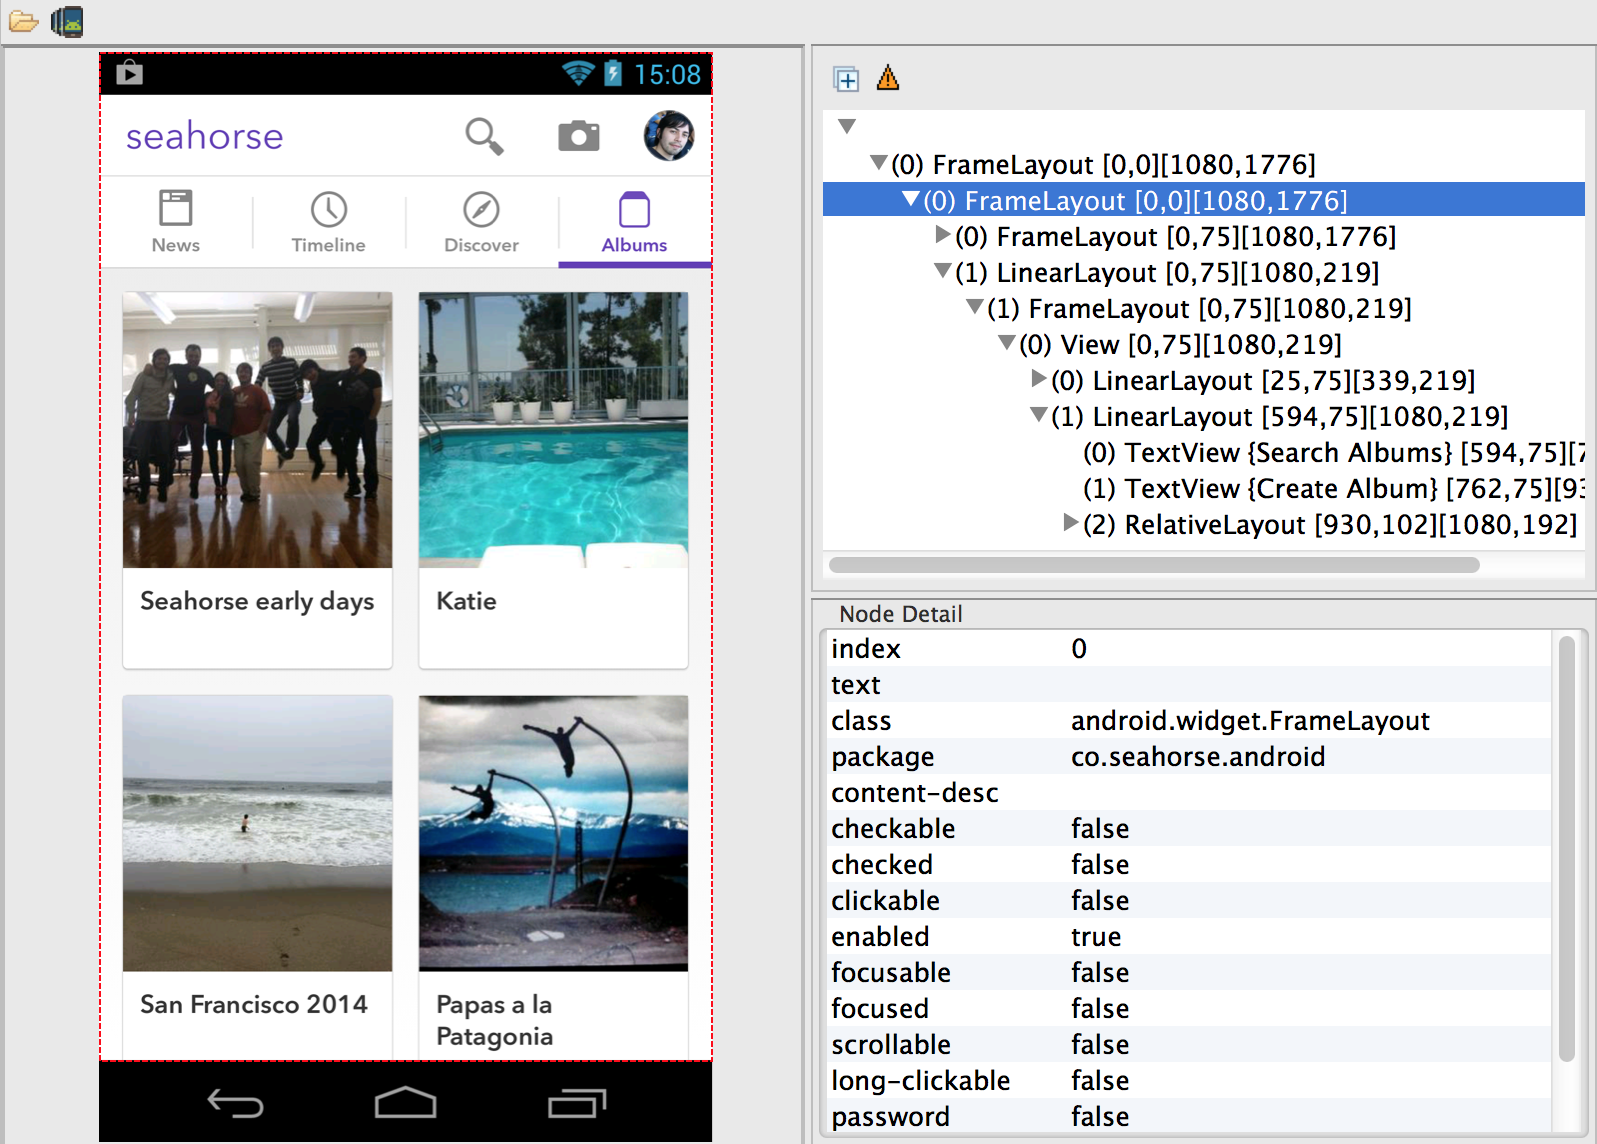
\includegraphics[width=15cm]{Imagenes/testing_uiautomatorview}
\caption{Vista de la herramienta uiautomatorviewer en una aplicaci�n. Fuente: Elaboraci�n Propia}
\label{fig:Fig19}
\end{figure}

\subsection{Monkey}
Esta herramienta es principalmente usada para realizar casos de testing de estr�s. Esto quiere decir que la aplicaci�n es deliberadamente sometida a una gran cantidad de eventos para determinar la estabilidad y el manejo de errores. Los eventos generados consistir�n en acciones que podr�a realizar un usuario normal, como clicks, toques, o gestos, pero en una cantidad muy elevada.\\

Por ejemplo, el siguiente comando enviar� 2000 eventos aleatorios a la aplicaci�n con el nombre de paquete \textit{co.seahorse.android}:\\

\begin{lstlisting}
adb shell monkey -p co.seahorse.android -v 2000
\end{lstlisting}

\section{Implementaci�n de Herramientas de Distribuci�n}
\subsection{HockeyApp}
Antes de HockeyApp, en Seahorse se usaba TestFlight \cite{59}, pero ellos dejaron de dar soporte a Android en Marzo de este a�o \cite{60} ya que fueron comprados por Apple, por lo que fue necesario migrar a otro servicio. HockeyApp cumpl�a con pr�cticamente todas las necesidades que entregaba TestFlight, siendo una de ellas el soporte para  aplicaciones tanto Android como iOS. 

Actualmente se pagan 10 d�lares por el servicio, de forma mensual, lo que corresponde al plan m�s econ�mico ofrecido por HockeyApp, que permite tener hasta 5 aplicaciones distintas en la plataforma con una cantidad ilimitada de usuarios.

Para distribuir las versiones, la primera vez es necesario agregar informaci�n b�sica como el nombre de la aplicaci�n y el nombre del paquete. Luego se sube el APK de la aplicaci�n y se invita a las personas que el desarrollador quiere que se conviertan en usuarios de prueba de esta versi�n. Cada vez que se sube una versi�n nueva, es posible notificar a los usuarios que ya cuentan con una versi�n anterior para que la actualicen. Adem�s, es posible invitar a nuevas personas en cualquier momento. 

El desarrollador cuenta con informaci�n b�sica de los testers, como el modelo y dispositivo con el que cuenta, y tambi�n es posible saber si es que ya tienen la �ltima versi�n.

En la figura \ref{fig:Fig22} se puede ver la vista que tiene el desarrollador sobre una versi�n beta de Seahorse. La acciones m�s frecuente est�n en la parte superior, teniendo opciones para subir una nueva versi�n de la misma aplicaci�n, invitar m�s usuarios o cambiar informaci�n b�sica de la aplicaci�n. En la parte inferior es posible ver la lista de todas las �ltimas versiones que se han enviado de esa aplicaci�n, con informaci�n como el peso de la aplicaci�n, cu�ndo fue subida esa actualizaci�n y la cantidad de descargas que se han tenido. En Seahorse no est� implementado el SDK de HockeyApp para la recepci�n de reporte de crashes, ya que se usa Crittercism, que entrega informaci�n m�s avanzada. Por �ltimo, sobre las acciones m�s frecuente hay un men� que ofrece la opci�n de ver todas las versiones que ha tenido la beta, la lista de usuarios que tienen acceso a la beta y el posible feedback que han entregado cada uno de ellos.
\begin{figure}
\centering
      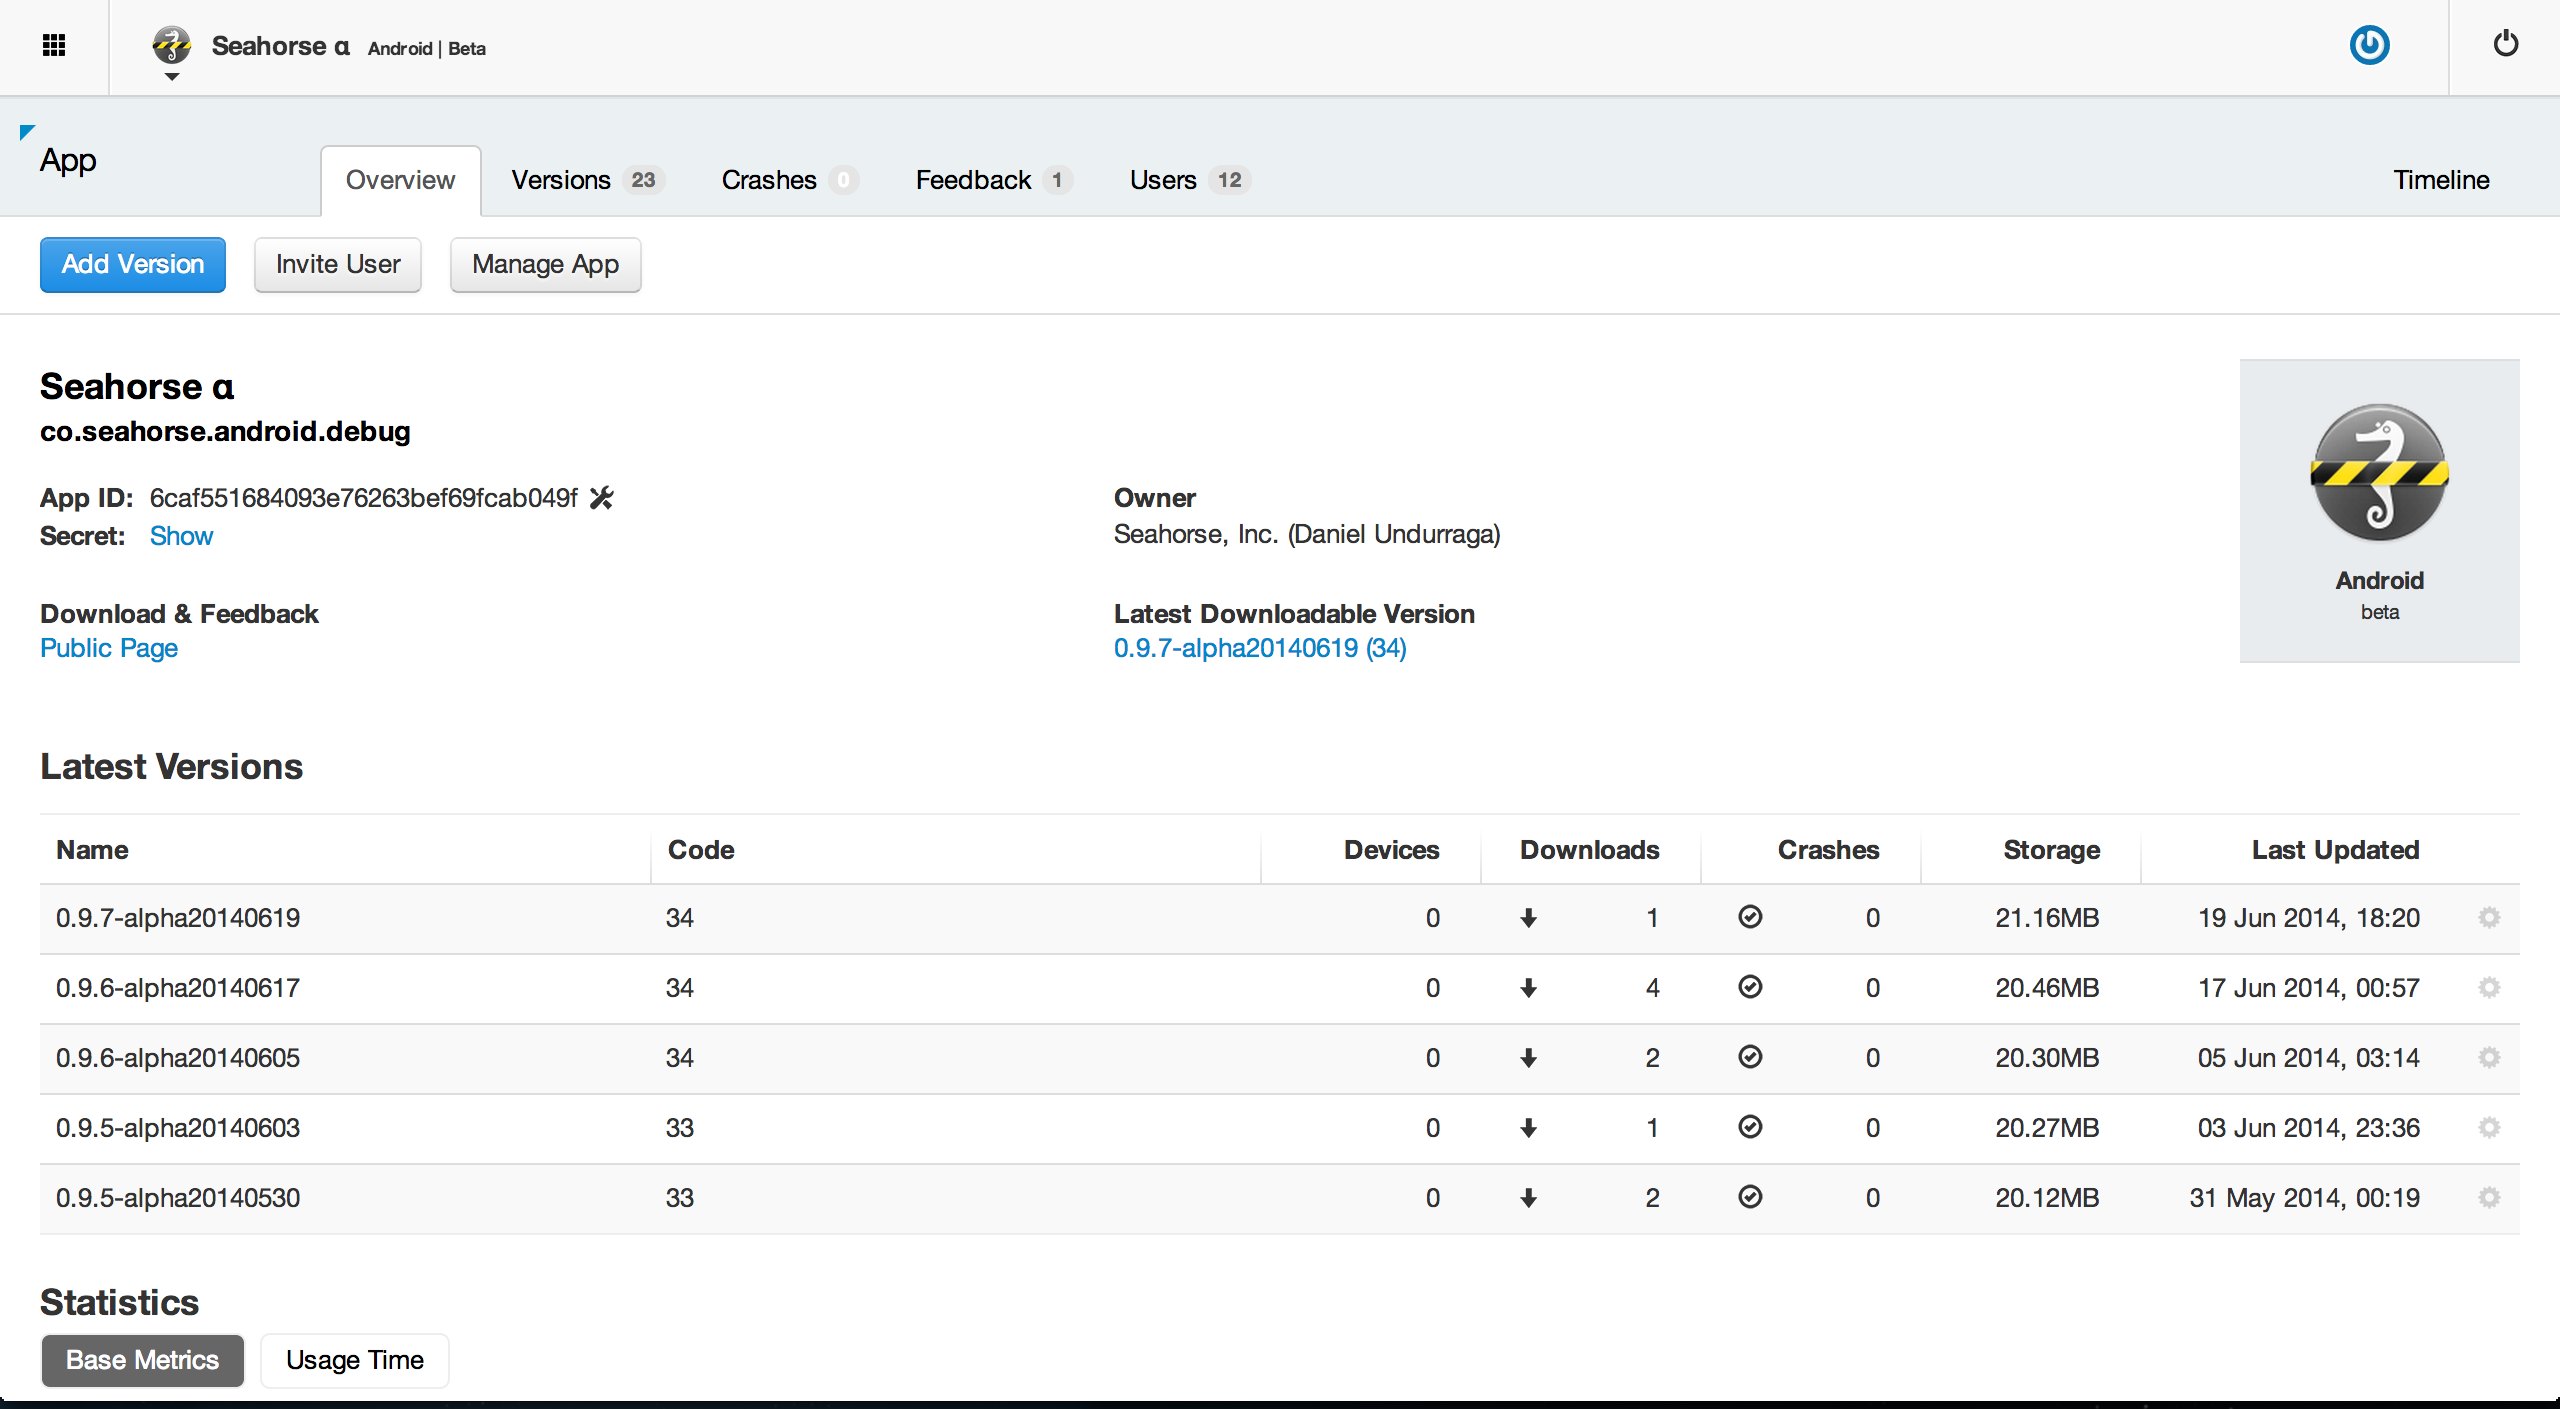
\includegraphics[width=15cm]{Imagenes/distribution_hockeyapp}
\caption{Vista de una aplicaci�n beta de Seahorse en HockeyApp. Fuente: Elaboraci�n Propia}
\label{fig:Fig22}
\end{figure}
%Para su implementaci�n es necesario crearse una cuenta dentro del sitio ....crear la app, subir apk, invitar gente al apk, dps de cada actualizacion aparece la lista de personas para notificarla, en la misma plataforma se puede ver el feedback que dan los usuarios.

\subsection{UserTesting}
UserTesting es la plataforma usada en Seahorse para lanzar versiones beta y recibir feedback de usuarios de prueba a trav�s de videos. Esta herramienta es usada por grandes empresas como Google, Apple, Microsoft, Twitter, Facebook y  Yahoo, para la distribuci�n y testing de versiones de prueba de sitios web, aplicaciones de escritorios y aplicaciones m�viles. El servicio funciona a trav�s de la compra de cr�ditos, en donde por ejemplo, 1000 d�lares otorgan al desarrollador 20 cr�ditos. Cada uno de estos cr�ditos sirve para realizar un test con un usuario, aunque tambi�n es posible realizar un mismo test a m�s de un usuario, pero en definitiva, por cada usuario que realice un test, un cr�dito es consumido. Debido al elevado valor de cada cr�dito, el desarrollador debe tener claro qu� es lo que quiere testear dentro de la aplicaci�n y cu�les son los resultados que espera.

En Seahorse se usa UserTesting al momento de implementar nuevas caracter�sticas en la aplicaci�n, para ver temas de usabilidad y para corroborar que el usuario entiende de forma intuitiva lo implementado. Adem�s sirve para encontrar posibles errores en otros dispositivos, ya que debido a la fragmentaci�n existente en Android es pr�cticamente imposible saber c�mo una aplicaci�n se ve en cada uno de los dispositivos existentes.

Para la creaci�n de un test los pasos son los siguientes:
\begin{itemize}
\item Seleccionar si la aplicaci�n m�vil es de Android o iOS

\item Agregar instrucciones de c�mo instalar la aplicaci�n y una breve descripci�n para que el usuario tenga una idea de lo que va a testear.

\item Agregar una serie de tareas que el usuario debe ir realizando. Tambi�n se pueden incluir preguntas durante el proceso, para saber si la tarea solicitada fue complicada, o simplemente para saber qu� piensa el usuario sobre esa tarea.

\item Agregar un cuestionario final con preguntas m�s generales sobre la aplicaci�n y el proceso completo.

\item Por �ltimo es posible solicitar algunas caracter�sticas demogr�ficas como el rango de edad, el pa�s, el g�nero, la experiencia con aplicaciones m�viles, y otras restricciones como versi�n de Android mayor a 4.0, o que el usuario cuente con fotos en su galer�a.
\end{itemize}

Cuando en Seahorse se agreg� el registro de usuarios a trav�s de Facebook y de Google+, se llev� a cabo la distribuci�n y testing a trav�s de esta plataforma. Esto permiti� corroborar que esta nueva caracter�stica, al igual que otras, funcionaban correctamente. Fue necesario hacer en total unos 8 tests, ya que en cada iteraci�n se usaban 4 cr�ditos, 2 para comprobar que el registro a trav�s de Facebook funcionaba bien, y otros 2 para comprobar lo mismo, pero a trav�s de Google+. Los tests a trav�s de Facebook funcionaron correctamente, pero con Google+ existieron dificultades, ya que uno de los usuarios no pudo realizar el registro. Debido a esto, despu�s de realizar algunas correcciones se llevaron a cabo nuevos tests, con los que se obtuvieron resultados positivos. Tal como se mencion� antes, es necesario aprovechar cada uno de los tests, por lo que adem�s de testear el registro de los usuarios, tambi�n se solicitaron otras tareas, como importar albums de otras plataformas, sincronizar la c�mara del dispositivo con Seahorse, invitar a otros usuarios a la aplicaci�n, entre otras cosas.

Cada uno de los videos entreg� informaci�n valiosa sobre la usabilidad dentro de la aplicaci�n, y permiti� verificar la UI en 8 dispositivos distintos, algunos con una pantalla muy peque�a. Si bien, la cantidad de tareas que se pueden solicitar a los usuarios no tiene l�mite, los tests deber�an durar alrededor de 15 minutos, ya que el sitio les paga a los usuarios por 15 minutos de video. Esto no quiere decir que si el test dura m�s de ese tiempo, no va a hacer v�lido, pero va a depender m�s de la voluntad del tester si desea seguir grabando 20 o 25 minutos. El usuario va relatando todo el proceso, desde la instalaci�n de la aplicaci�n, hasta el cuestionario final.

\section{Implementaci�n de Herramientas de Reportes de Crashes}
\subsection{Crittercism}
Crittercism ha sido la plataforma escogida para la recepci�n de crashes, principalmente por el nivel de detalle presente en sus reportes. Adem�s el valor que se paga mensualmente es bastante accesible para cualquier empresa del rubro. Actualmente dentro de Seahorse, se pagan 24 d�lares mensuales por este servicio, lo que da acceso a reportes muy detallados que permiten reparar de forma r�pida cada crash. 

Crittercism ha permitido disminuir la tasa de crashes y ofrece variadas estad�sticas para ver informaci�n sobre los dispositivos en los que existen m�s crashes, el sistema operativo en que ocurren m�s crashes o la versi�n en la que ocurrieron m�s crashes. Despu�s del lanzamiento de cada actualizaci�n se reparan una gran cantidad de bugs, pero aparecen nuevos crashes, lo que es inherente al proceso de desarrollo de software, ya que se incluye nuevo c�digo, pero con esta herramienta es posible contar con informaci�n muy detallada, facilitando en gran medida la tarea de los desarrolladores.

La instalaci�n es bastante simple \cite{31}. Para agregar Crittercism a un proyecto configurado con Gradle es necesario agregar esta l�nea al archivo \textit{build.gradle} del proyecto:
\begin{lstlisting}
compile 'com.crittercism:crittercism-android-agent:+'
\end{lstlisting}
Luego se deben agregar estos permisos en el Android Manifest del proyecto: 
\begin{lstlisting}
<uses-permission android:name="android.permission.INTERNET"/>
<uses-permission android:name="android.permission.READ_LOGS"/>
<uses-permission android:name="android.permission.ACCESS_NETWORK_STATE"/>
<uses-permission android:name="android.permission.GET_TASKS"/>
\end{lstlisting}
El primer permiso es necesario para poder acceder a Internet y poder enviar los reportes. El segundo es necesario para poder obtener la informaci�n de los stack trace del usuario, y ahi saber en qu� l�nea de c�digo ha ocurrido el error. El tercero es para obtener informaci�n sobre el estado de la red, por ejemplo, para saber si el usuario est� conectado a Wi-Fi o a trav�s de un carrier. El �ltimo permiso sirve para acceder a la informaci�n de las �ltimas dos \textit{Activities} ejecutadas, lo que permite saber en qu� pantalla ocurri� el crash.

Una vez que los permisos ya est�n entregados, se debe inicializar Crittercism. Esto se hace �nicamente una vez por aplicaci�n, por lo que se debe hacer en la primera \textit{Activity} que se ejecuta dentro de la aplicaci�n. Para iniciar Crittercism se escribe la siguiente l�nea en el onCreate:
\begin{lstlisting}
Crittercism.initialize(getApplicationContext(), "CRITTERCISM_APP_ID");
\end{lstlisting}

Ahora ya est�n implementadas las caracter�sticas b�sicas, y comenzar�n a llegar los reportes al sitio web de Crittercism. Tambi�n es posible agregar a otros desarrolladores al servicio, para que tengan acceso a la misma informaci�n y que todo el equipo reciba los reportes de crashes al correo.

La documentaci�n con la que cuenta es excelente para entender los alcances y todas las cosas que se pueden hacer a trav�s de Crittercism. Por ejemplo, es posible recibir las excepciones que ocurren dentro de la aplicaci�n. Esto se realiza agregando las siguientes l�neas en la excepci�n que se desea recibir:
\begin{lstlisting}
try {
    throw new Exception("Aqu� ocurre una excepci�n");
} catch (Exception exception) {
    Crittercism.logHandledException(exception);
}
\end{lstlisting}

A trav�s de los gr�ficos de la figura \ref{fig:Fig23} es posible dimensionar la utilidad de contar con una herramienta como Crittercism. El gr�fico de la izquierda indica la cantidad de reportes de crashes recibidos por distintas versiones de la aplicaci�n durante el mes de Enero. El gr�fico de la derecha indica la cantidad de usuarios que han sido afectados por al menos un crash durante ese mismo per�odo. A trav�s de estos gr�ficos es posible ver que la versi�n 0.8.8 de color amarillo, fue lanzada el d�a 9 de Enero y r�pidamente comenzaron a llegar una gran cantidad de reportes de crashes, alcanzando la cifra de 173 crashes y afectando a m�s de 100 usuarios. Debido a ello, al d�a siguiente se lanz� la versi�n 0.8.8.1 de color verde, la cual se encarg� de arreglar el error introducido en la versi�n previa y reduciendo este n�mero en gran medida, con s�lo 35 crashes y afectando a 20 usuarios. Si esta herramienta, probablemente habr�an transcurrido m�s d�as con el mismo problema, afectando a muchos m�s usuarios. 
\begin{figure}
\centering
      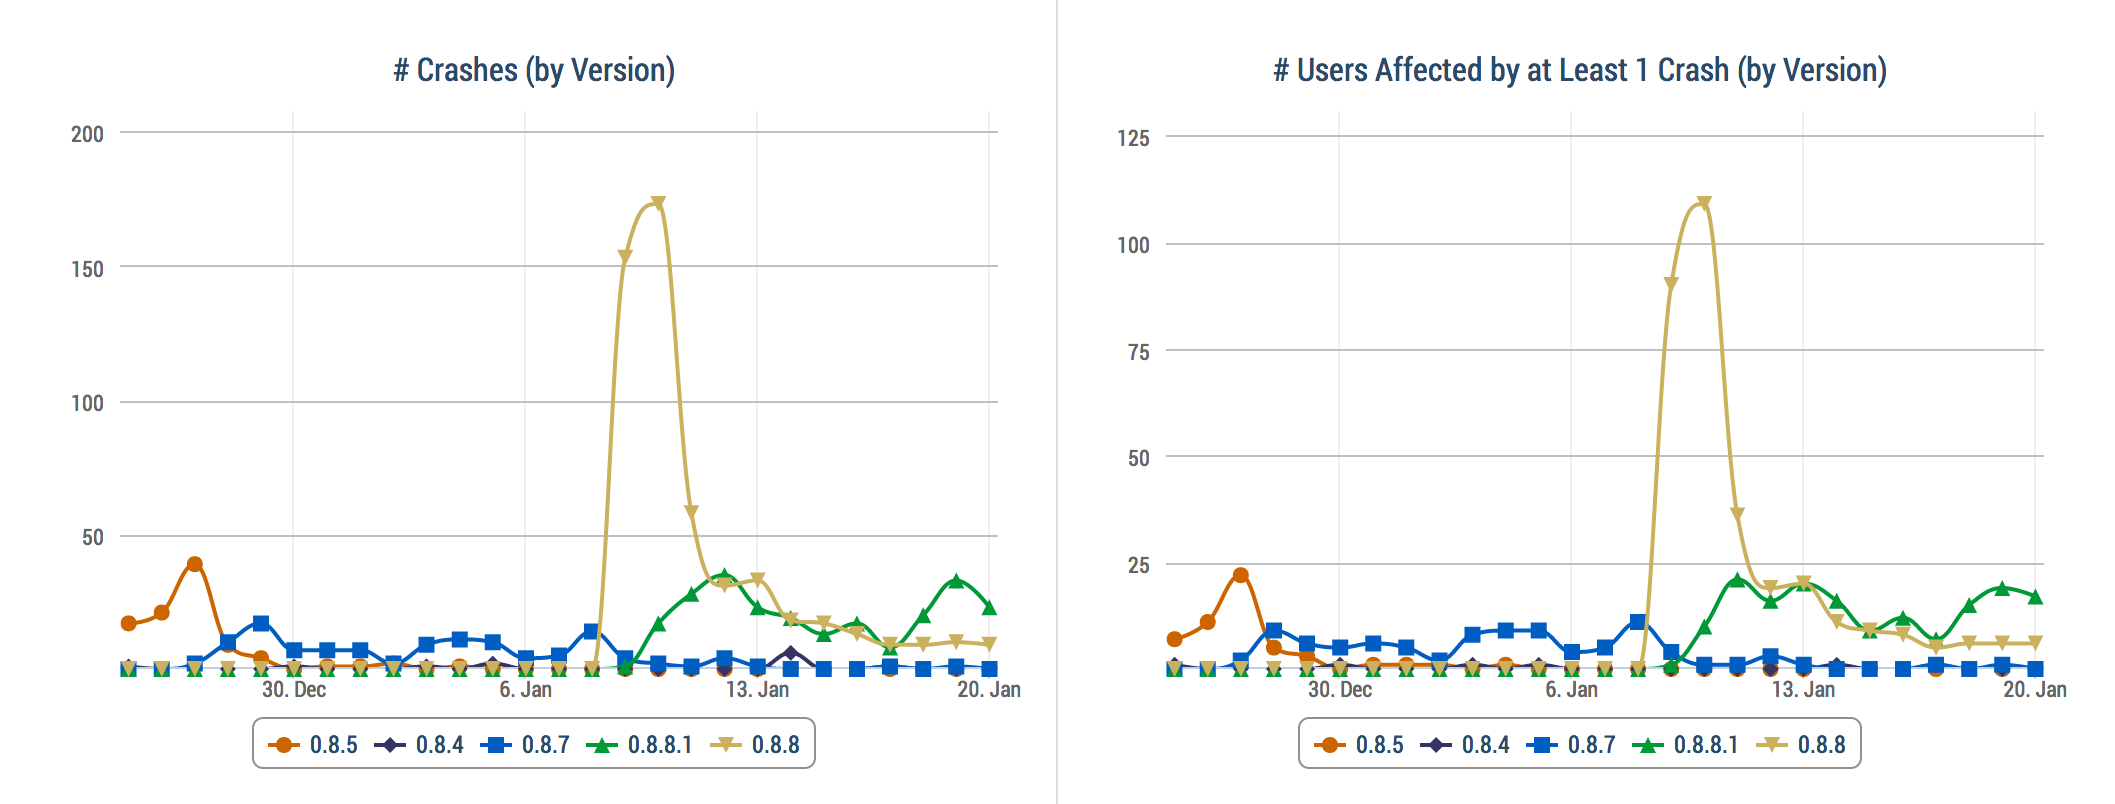
\includegraphics[width=14cm]{Imagenes/crash_report_crittercism_graphs}
\caption{Gr�ficos que entrega Crittercism sobre cantidad de crashes y usuarios afectados en un periodo de un mes. Fuente: Elaboraci�n Propia}
\label{fig:Fig23}
\end{figure}

%\subsection{Google Analytics}
%Google Analytics ha sido implementada, aunque no por sus reportes de crashes, sino que para el tracking de eventos y performance.
%Para su implementaci�n es necesario descarga desde el sitio de Google Analytics \cite{33} la versi�n 3 de su SDK. Una vez descargado el SDK, es necesario incluirlo al proyecto y dar los siguientes permisos en el archivo Android Manifest:
%\begin{lstlisting}
%<uses-permission android:name="android.permission.INTERNET"/>
%<uses-permission android:name="android.permission.ACCESS_NETWORK_STATE"/>
%\end{lstlisting}
%Para implementarlo a trav�s de c�digo es necesario agregar estas l�neas en cada una de las \textit{Activities} de las cu�les se desee obtener informaci�n:
%\begin{lstlisting}
%@Override
%  public void onStart() {
%    super.onStart();
%    ... // El resto del c�digo de onStart()
%    EasyTracker.getInstance(this).activityStart(this);  // Agregar este m�todo
%  }

%  @Override
%  public void onStop() {
%    super.onStop();
%    ... // El resto del c�digo de onStop()
%    EasyTracker.getInstance(this).activityStop(this);  // Agregar este m�todo
%  }
%\end{lstlisting}
% ---------------------------------------------------------------------------------------------------------------
% Cap�tulo 5: Conclusiones y Trabajo Futuro
% ---------------------------------------------------------------------------------------------------------------
\chapter{Conclusiones}
\label{ch:conc}
\section{Conclusiones Generales}
A trav�s de este trabajo, se han estudiado y comparado diversas herramientas que ayudan a mejorar la calidad de las aplicaciones desarrolladas para Android. 

Esto se ha llevado a cabo identificando los problemas existentes durante el desarrollo de aplicaciones m�viles, dejando en evidencia que el elemento que m�s afecta al sistema operativo Android es la fragmentaci�n en dos niveles: software y hardware. De esta �ltima, se desglosan la mayor�a de los problema inherentes a la inmensa cantidad de dispositivos que existen, como por ejemplo los distintos tama�os y resoluciones de pantalla. Tambi�n existen diferencias de RAM, espacio, n�cleos y procesador en cada uno de los dispositivos. Por otro lado, existen problemas que est�n m�s relacionados con el proceso de desarrollo de software. Entre �stos se encuentran la distribuci�n de versiones betas que permiten probar con usuarios reales una aplicaci�n antes de que �sta se encuentre disponible para descargar de forma oficial. El �ltimo problema se enfrenta cuando la aplicaci�n ya se encuentra en la tienda oficial de Google, y no se sabe realmente si la aplicaci�n est� respondiendo como se espera o est� presentando errores.

Para atacar cada uno de estos problemas es necesario contar con herramientas que permitan darle un grado de seguridad al desarrollador de que todo va a funcionar de forma correcta, y que en cierto modo, aseguren la calidad de la aplicaci�n desarrollada. Es por ello que se buscaron herramientas que solucionan o al menos mitigan los problemas presentados anteriormente. La Fragmentaci�n de Android no es un problema que se pueda solucionar con una herramienta, ya que por ejemplo es inviable probar una aplicaci�n en los m�s de 11.000 dispositivos existentes, y en cada una de las 8 versiones de Android que se encuentran vigentes, por lo que la �nica forma de combatir y mitigar la fragmentaci�n es a trav�s del testing, tanto automatizado como manual. Por otro lado, la distribuci�n de versiones y los crashes son problemas que son solucionables en su totalidad con herramientas que permiten realizar estas tareas. Es por ello que las herramientas fueron clasificadas en tres categor�as: Testing, Distribuci�n de Versiones y Reportes de Crashes.  

Para cada una de las categor�as se realiz� un an�lisis comparativo, a trav�s del cual se definieron las ventajas y desventajas de cada una de las herramientas. En algunos casos fue necesario subdividir las categor�as para que las comparaciones entreguen resultados m�s valiosos. Esto permite que los desarrolladores cuenten con informaci�n relevante para tomar mejores decisiones al momento de tener que implementar una de estas herramientas. 

En base a las caracter�sticas de cada herramienta, se han implementado algunas de ellas en una aplicaci�n que est� disponible en la tienda oficial de Google. Cabe mencionar que las herramientas implementadas fueron las que se ajustaban m�s a las necesidades de la aplicaci�n Seahorse. Es posible que otros desarrolladores, en base a las ventajas y desventajas presentadas, implementen otro conjunto de herramientas que se ajuste m�s a su contexto.

Adem�s, se descubri� que la gran cantidad de documentaci�n encontrada estaba obsoleta. Esto se debe principalmente al r�pido desarrollo que ha tenido el sistema operativo Android, por lo que algunas bibliotecas que llevan a�os de desarrollo simplemente no actualizan su documentaci�n. Otro de los puntos importantes es que hoy en d�a los desarrolladores est�n divididos entre el uso de Eclipse como IDE, y el uso de IntelliJ, que son los dos IDE recomendados para el desarrollo de aplicaciones para Android, aunque poco a poco los desarrolladores deber�an ir inclin�ndose m�s por este �ltimo, ya que Google esta promoviendo m�s su uso a trav�s de caracter�sticas que facilitan tanto el dise�o de interfaces, como la escritura, autocompletaci�n y refactorizaci�n de c�digo. El hecho de que existan dos IDE genera que la documentaci�n se encuentre a�n m�s obsoleta, ya que la mayor�a solo cubre la integraci�n con Eclipse.

\section{Conclusiones Espec�ficas}
\begin{itemize}
\item La mayor�a de la documentaci�n de las herramientas de testing s�lo cubren la integraci�n con Eclipse, por lo que si reci�n se est� comenzando a desarrollar un proyecto, y se tiene que elegir entre Eclipse o Android Studio para iniciar el desarrollo, es recomendable usar la primera. Si bien Android Studio se basa en IntelliJ, la versi�n modificada por Google especialmente para el desarrollo de aplicaciones Android lleva poco m�s de un a�o de desarrollo y a�n se encuentra en versi�n beta, por lo que le falta bastante para acercarse a la robustez y madurez ofrecida por Eclipse.

\item Si se desea comenzar a hacer testing unitario dentro de una aplicaci�n Android, se recomienda desarrollar la mayor cantidad de c�digo independiente de la API de Android, ya que los test se ejecutar�an en la m�quina virtual de Java. En los casos en que el c�digo dependa de la API de Android, los tests igualmente pueden ser ejecutados en la m�quina virtual de Java gracias a Robolectric, aunque estos tomar�n un poco m�s de tiempo que los tests que tienen s�lamente c�digo Java. Si el c�digo que se desea testear cuenta con muchas llamadas a la API de Android, puede que sea necesario usar el Framework de Testing de Android, y estos tests tomar�n mucho m�s tiempo, ya que es necesario ejecutarlos en un dispositivo o un emulador con Android.

\item Si se desea comenzar a hacer testing de la interfaz gr�fica de una aplicaci�n Android, la herramienta a utilizar va a depender principalmente de lo que se quiera testear. Si se quieren testear casos en que una aplicaci�n interact�a con la aplicaci�n de la c�mara o con otras aplicaciones, eso es posible con la herramienta nativa, uiautomator. En caso contrario, tanto Robotium como Espresso son muy buenas herramientas. La gran ventaja de Robotium son los 4 a�os de desarrollo con los que cuenta, acompa�ado de excelente documentaci�n. Por otro lado, si bien Espresso es una herramienta nueva y a�n no cuenta con una gran comunidad, los tests ejecutados con Espresso son tres veces m�s r�pidos que Robotium, ya que est�n sincronizados con el \textit{thread} de la UI.

\item La elecci�n de una de las herramientas de distribuci�n de versiones va a depender del grado de distribuci�n que se est� buscando. Si se desea distribuir versiones beta de forma masiva, la opci�n para ello es Google Play Console. Para grupos peque�os, con los que se busca tener una relaci�n m�s cercana y recibir feedback constante, est�n HockeyApp y AppBlade. Por �ltimo est�n UserTesting y The Beta Family, que entregan la opci�n de distribuir una versi�n beta y que los usuarios realicen testing manual de la aplicaci�n, a trav�s de una serie de tareas y preguntas especificadas por el desarrollador. Si bien, la mayor�a de estas herramientas ofrecen una opci�n gratuita, para acceder a las caracter�sticas m�s relevantes es necesario pagar, por lo que la decisi�n puede depender del presupuesto del desarrollador. 

\item Para elegir una herramienta que entregue reporte de crashes el desarrollador debe fijarse en el nivel de detalle que quiere recibir. Las herramientas que entregan una mayor cantidad de informaci�n son Crittercism y Bugsense, aunque son de pago. Las opciones gratuitas son Google Analytics, que entrega informaci�n b�sica sobre los crashes y estad�sticas generales de la aplicaci�n, aunque los reportes tienen un retraso de un d�a, y ACRA, que permite especificar qu� informaci�n se desea recibir en cada reporte, aunque la desventaja est� en que el desarrollador debe implementar su propio servicio web para visualizar los reportes.
\end{itemize}


\section{Trabajo Futuro}
Si bien se tomaron como punto de referencia herramientas que solucionan o mitigan los problemas comunes al desarrollar aplicaciones Android, existen otras herramientas que tambi�n podr�an mejorar la calidad de las aplicaciones, y que est�n esperando a ser analizadas y popularizadas por los desarrolladores como Appurify, Testdroid, AppThwack, entre muchas otras. Adem�s, las comunidades de herramientas de c�digo abierto son muy activas y se encargan de mantenerlas actualizadas, mejor�ndolas de forma peri�dica.

Considerando el alcance de esta memoria, fueron dejadas para estudios futuros herramientas como las siguientes:
\begin{itemize}
\item Herramientas de debugging y an�lisis de performance como Traceview, Systrace, Monitor, DDMS, todas excelentes herramientas ofrecidas por Android de forma nativa.

\item Herramientas de an�lisis de datos y tracking de eventos como Mixpanel, Flurry, Google Analytics, etc.

\item Herramientas de apoyo a bases de datos como ORMLite, GreenDAO, etc.

\item Bibliotecas �tiles para el desarrollo en Android como Picasso, Universal Image Loader, Volley, GSON, Jackson, entre otras.
\end{itemize}

% ---------------------------------------------------------------------------------------------------------------

\appendix
%!TEX root = ../tesis.tex
% Ap?dice A: 
% ---------------------------------------------------------------------------------------------------------------
%\chapter{Ap?dice A}
%\label{ch:apeA}

%\section{Secci? Ap?dice}
%\label{sec:SecApe}

% ---------------------------------------------------------------------------------------------------------------
% ---------------------------------------------------------------------------------------------------------------
\singlespacing
\bibliographystyle{plain}
\bibliography{manual} %Use Mendeley Tool or automatic creation (http://mendeley.com)
% ---------------------------------------------------------------------------------------------------------------
\end{document} 